\begin{refsection}[research/yunoki/group.bib]
\nocite{*}
\chapter{Computational Materials Science Research Team}

\section{Members}

\begin{itemize}
  \item[] Seiji Yunoki (Team Leader)
  \item[] Yuichi Otsuka (Research Scientist)
  \item[] Shigetoshi Sota (Research Scientist)
  \item[] Shixun Zhang (Postdoctoral Researcher)
  \item[] Ahmad Ranjbar (Postdoctoral Researcher)  
  \item[] James S. M. Anderson (Foreign Postdoctoral Researcher)  
  \item[] Kazuhiro Seki (Special Postdoctoral Researcher, joint)  
  \item[] Sandro Sorella (Senior Visiting Scientist)
  \item[] Takami Tohyama (Senior Visiting Scientist)
  \item[] Yutaka Imamura (Visiting Scientist)
  \item[] Susumu Yamada (Visiting Scientist)
  \item[] Michele Casula (Visiting Scientist)  
  \item[] Keiko Matsuoka (Assistant)  
\end{itemize}

\section{Research Activities}

The main purpose of our team is to understand and predict quantum states of condensed matter systems and 
solid state materials for the next generation highly functional materials and for the basis of future revolutionary 
technologies. More emphasis is put specially on strong many-body correlations that require the treatment going 
beyond the single-particle approximation. For this purpose, we develop many-body numerical methods, which 
include numerically exact diagonalization method, classical Monte Carlo and molecular dynamics methods, 
quantum Monte Carlo method, and density matrix renormalization group method. We also develop highly 
parallelized application software based on these numerical methods to efficiently perform large-scale simulations.

\section{Research Results and Achievements}

\subsection{Development of large-scale quantum Monte Carlo (QMC) simulations}

The QMC method is one of the most powerful tools to investigate quantum many-body systems. There are 
several variants of QMC techniques depending on target systems. Among them, we have developed the 
determinant Monte Carlo method to study the interacting fermions on lattice, i.e., the Hubbard model, with 
a specific aim to calculate physical observables with a high degree of accuracy on quite large systems. 
The accuracy and the system size are inseparable in the lattice simulations as the energy resolution is 
roughly determined by the inverse of the linear size L of the system. Therefore, it is inevitable to perform 
simulations on very large clusters in order to accurately calculate physical observables, which demands 
huge computational resources. Since the numerical calculations are based mostly on linear algebraic 
operations such as matrix-matrix product and numerical orthogonalization, we can take advantage of the 
highly optimized numerical library on K computer. We have also optimized the delayed update algorithm to 
efficiently use the cache memory. We have confirmed that our simulation code achieves 80\% of the peak performance in the single node calculation with increasing the system size (see Fig.~\localref{fig:qmc_pf}). 
Since in this case one Slater determinant, representing one ensemble in the Monte Carlo sampling, can be 
stored in the single node, we are able to use up to 24,576 nodes with quite high efficiency of about 50\% 
of the peak performance in total. We have utilized this code in the practical study of the two-dimensional (2D) 
Hubbard model on honeycomb lattice with the system size up to $N=2,596$ sites, which is about 4 times larger 
than the previous study ($N=648$) [Z. Y. Meng et al., Nature {\bf 464}, 847 (2010)] and represents currently 
the largest system size ever. The computational complexity scales as $N^3$ and thus it could have not been 
possible without K computer. We have also implemented more non-trivial parallelization for the case where one 
Slater determinant is distributed to a group of multiple nodes, in which the parallelized numerical library 
ScaLAPACK is employed to update the Slater determinant in each Monte Carlo sweep. With this 
implementation, it has become possible to perform the simulations with $N$ up to 8,100 within reasonable 
CPU time.

\begin{figure}
\centering
  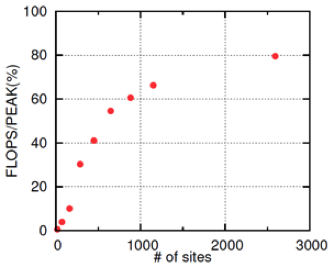
\includegraphics[width=0.5\textwidth,keepaspectratio,natwidth=193,natheight=40]
  {research/yunoki/qmc_pf.png}
  \caption{Peak performance of benchmark calculations for the Hubbard model with various system sizes.}
  \locallabel{fig:qmc_pf}
\end{figure}


\subsection{Absence of spin liquid in the half-filled Hubbard model on the honeycomb lattice}

First, we have applied our improved QMC code to elucidate the ground state phase diagram of the half-filled 
Hubbard model on the honeycomb lattice model (honeycomb lattice model), in which a gapped spin liquid (SL) 
phase was proposed previously [Z. Y. Meng et al., Nature {\bf 464}, 847 (2010)]. Since it is widely believed that 
not only strong quantum fluctuations but also geometrical frustrations are responsible for stabilizing a SL phase, 
the possibility of SL phase in the unfrustrated honeycomb lattice is rather surprising, and thus has been one of 
the most debated issues in recent years. The proposed SL phase in the previous report was claimed to exist 
for $3.4 < U/t < 4.3$ ($U$: Hubbard interaction, $t$: nearest neighbor hopping) as a spin-gapped insulating 
phase without any broken symmetry. We thus have first tried to clarify the existence of SL at $U/t = 4$, which 
corresponds to the middle of the proposed SL region. Taking a full advantage of K computer, we have 
performed the QMC simulations on the lattice with $N=2L^2$ up to 2,596 sites. Figure~\localref{fig:qmc_sc} 
shows our results of the antiferromagnetic (AF) spin structure factors, $S_{\rm AF}$, and spin-spin correlation 
functions at the maximum distance, $C_s (L_{\rm max})$, at $U/t=4$. The extrapolated values of both quantities 
are confirmed to be finite within statistical errors, indicating the AF long-range order. Complemented with 
simulations performed at other $U/t$, our results strongly support the conventional scenario that a single and 
direct phase transition occurs between semi-metal and antiferromagnetic Mott insulator with increasing $U/t$. 


\begin{figure}
\centering
  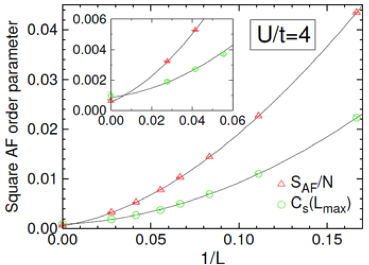
\includegraphics[width=0.5\textwidth,keepaspectratio,natwidth=193,natheight=40]
  {research/yunoki/qmc_sc.png}
  \caption{Finite size scaling of AF order parameter squared at $U/t=4$.}
  \locallabel{fig:qmc_sc}
\end{figure}


\subsection{Quantum criticality of metal-insulator transition in 2D interacting Dirac electrons}

Next, having established the continuous character of the transition, we have performed careful finite-size scaling 
analysis of our QMC data to obtain critical exponents of this metal-insulator transition. 
As shown in Fig.~\localref{fig:qmc_cp}, the data of the staggered magnetization calculated on finite-size clusters 
are excellently collapsed into a universal function in the honeycomb lattice model and also the Hubbard model on 
square lattice with a magnetic flux $\pi$ per plaquette ($\pi$-flux model). The latter model is known to have 
massless Dirac dispersions as in the honeycomb lattice model. It is turned out that the critical exponents are 
exactly the same within the statistical errors for the two lattice models, which strongly suggests that the 
metal-insulator transitions in these models belong to the same universality class. This class should be coincident 
with that in the Gross-Neveu model, a model extensively studied in the particle physics, since it has recently 
been recognized that the effective model for the 2D interacting Dirac fermions in the continuous limit is described 
by the Gross-Neveu model. Thus, we expect that our finding based on the unbiased large-scale QMC 
simulations have an impact also in an interdisciplinary field.

\begin{figure}
\centering
  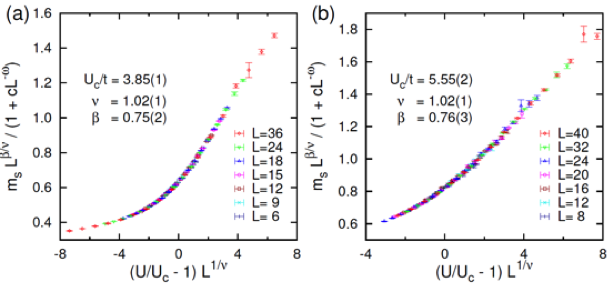
\includegraphics[width=0.5\textwidth,keepaspectratio,natwidth=193,natheight=40]
  {research/yunoki/qmc_cp.png}
  \caption{Data collapse fits for (a) honeycomb lattice and (b) $\pi$-flux models.}
  \locallabel{fig:qmc_cp}
\end{figure}


\subsection{Development of massively parallel density matrix renormalization group (DMRG) algorithms}

The DMRG method was originally proposed by S. White in 1992. Although the DMRG method was soon 
recognized as one of the best numerically exact methods for strongly correlated many-body quantum systems, 
the application is severely limited mostly to one-dimensional (1D) systems because of the exponential increase 
of degrees of freedom in higher spatial dimensions. However, owning to high performance computers that are 
recently availably, it has become realistic to apply the DMRG method even to 2D systems. We have been 
developing massively parallel DMRG algorithms to investigate strongly correlated quantum systems in two 
dimensions. We have already successfully developed our massively parallel DMRG code that employs many 
efficient parallelization techniques, and the first version of our massively parallel DMRG code has been opened 
in public for general users of K computer. A typical performance of the present version of our massively parallel 
DMRG code is summarized in Fig.~\localref{fig:dmrg_et}. For this example, we have calculated the optical 
conductivity for the 1D Hubbard model, using K computer with up to 82,488 nodes. We have performed the 
dynamical DMRG calculations with the DMRG truncation number $m=8,064$ 
(the number of bases kept during the calculation). 
The energy parallelization number is varied in such a way to correspond to the week scaling. 
As shown in Fig.~\localref{fig:dmrg_et}, we have achieved the extremely high peak performance ratio of 
73.6\% when 82,488 nodes are used on K computer, which is about 7.8 PFLOPS. 

\begin{figure}
\centering
  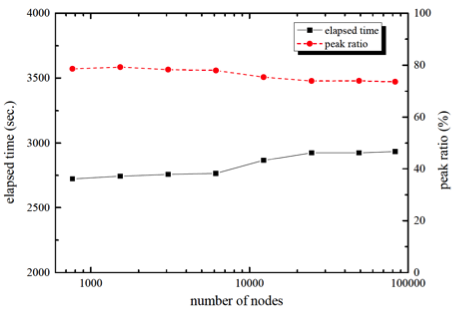
\includegraphics[width=0.5\textwidth,keepaspectratio,natwidth=193,natheight=40]
  {research/yunoki/dmrg_et.png}
  \caption{Performance of our massively parallel DMRG code on K computer.}
  \locallabel{fig:dmrg_et}
\end{figure}


\subsection{Magnetic excitations of the doped Hubbard model in two dimensions: Dynamical DMRG study} 

In order to disentangle magnetic excitations in the resonant inelastic X-ray scattering (RIXS) spectrum for 
electron-doped high-Tc cuprate Nd$_{2-x}$Ce$_x$CuO$_4$ ($x$: electron doping rate from half filling), 
we have performed the dynamical DMRG calculations using our massively parallel DMRG code on K computer. 
It has been reported experimentally that the peak position corresponding to the magnetic excitation in the 
RIXS spectrum sifts toward higher energy with increasing doping rate $x$ 
[K. Ishii, et. al., Nat. Commun. {\bf 5}, 3714 (2014)]. To understand this unexpected doping dependence, 
we have calculated dynamical spin structure factor $S({\bf q},\omega)$ for one of the simplest models for the 
high-Tc cuprate , i.e., the 2D Hubbard model with long range hoppings on the square lattice. Using K computer, 
we were able to do the calculations for clusters up to 6x6 sites, which represents currently the largest dynamical 
calculations in the world for the Hubbard model away from the half filling. We have found that the lowest peak in 
the dynamical spin structure factor $S({\bf q},\omega)$ shift toward higher energy with electron doping, thus in 
good qualitative agreement with the RIXS observation.


\subsection{Time-dependent DMRG method for real time quantum dynamics in two dimensions} 

Up to now, no reliable numerical method has existed for the real time dynamics of 2D strongly correlated 
quantum systems. We have challenged this issue by extending our massively parallel DMRG method combined 
with the kernel polynomial expansion. The previously proposed time-dependent DMRG method employs the 
Suzuki-Trotter decomposition for the time evolution operator $e^{i\delta t\hat H}$. 
Although this scheme costs computationally quite small since the time-evolution operator is given a product of 
local operators, it is limited only to 1D systems. Therefore, we have proposed a new time-dependent DMRG 
method combined with the kernel polynomial expansion to calculate directly the time evolution operator in any 
spatial dimension. Employing Legendre polynomials $P_l (x)$, the time-evolved state at $T=t+\delta t$ 
is given as $|t+\delta t\rangle = \lim_{L\to\infty}\sum_{l=0}^\infty (-i)^l (2l+1) j_l(\delta t) P_l(\hat H) |t\rangle$, 
where $j_l (x)$ is a spherical Bessel function. Since the special functions are satisfied with the three-term 
recursive formula, the time-evolved state is calculated recursively. In the practical calculation, we can truncate 
the number L of kernel polynomials to a finite value because the convergence of the kernel polynomial expansion 
is quite fast when $\delta t$ is small. With our new algorithm, we were successfully able to perform the reliable real 
time dynamics simulations in two dimensions for the first time. We have investigated, for example, the quantum 
annealing for the 2D Ising model with the time-dependent transverse magnetic field, a relevant system for 
quantum information.


\subsection{Development of ab-initio DMRG method for strongly correlated molecular systems}

Ab-initio DMRG method is developed in the quantum chemistry to perform the full configuration interaction 
(full-CI) calculations. Traditionally, the exact diagonalization method is used in the full-CI calculations. However, 
the degrees of freedom for strongly correlated molecular systems are quite large and increase exponentially 
with the number of orbitals considered. Thus, the exact diagonalization method is severely limited to small 
molecules. To overcome this difficulty, we have been developing massively parallel ab-initio DMRG method 
for the full-CI calculations. The computational complexity depends strongly on the connectivity of the system, 
which relates to the area-low of the entanglement entropy of the quantum state, and thus the order of the 
orbitals is crucial for the efficient ab-initio DMRG calculations. We have developed a general scheme to give 
the most efficient order of the orbitals in the DMRG calculation by using the graph theory. This allows us to 
perform the ab-initio DMRG calculations without explicitly considering the orbital order. Our ab-initio DMRG 
method has been extended for the dynamical calculations using the dynamical DMRG method.


\subsection{Magnetic Skyrmions in chiral magnets: Electrons coupled with classical spins}


Spins in chiral magnetic materials such as MnSi with a non-centrosymmetric structure are modulated significantly 
by Dzyaloshinskii–Moriya (DM) interaction and thus exhibit complex spin texture. Notably, there exists a 
vortex-like spin configuration named Skyrmion that shows non-trivial topological properties such as topological 
Hall effect. Due to the potential application of Skyrmion in the future information storage, Skyrmion has attracted 
intensive attention in recent years. We have examined chiral magnetic structure including Skyrmion using 
Monte Carlo and molecular dynamics simulations.

  The first class of systems studied is modeled by the double exchange model where the classical spins are 
coupled to the non-interacting electrons described by a simple tight binding model. To simulate this model, 
we have developed a semi-quantum Monte Carlo method, in which the electron degrees of freedom are 
numerically solved exactly for a give spin configurations and the spin degrees of freedom are treated using 
the importance sampling. Because the system size N has to be large enough to accommodate many 
Skyrmions with typically tens of nanometers, the exact diagonalization of electron degrees of freedom requires 
huge computation cost of $O(N^3)$. Therefore, we have adopted a kernel polynomial method (KPM) to expand 
the electron Green’s function using Chebyshev polynomials, which reduces the computational complexity 
down to $O(N)$. Applying the KPM, we were able to simulate up to 10,000 electrons coupled with 10,000 
classical spins.  The Skyrmion phase digram with temerature vs magnetic field is shown in 
Fig.~\localref{fig:mc_sky}, which is in e
xcellent agreement with experimental observations.


\begin{figure}
\centering
  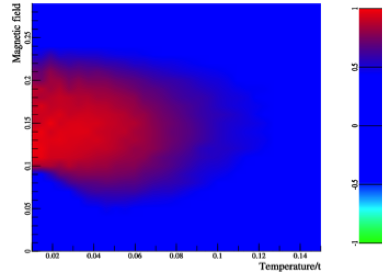
\includegraphics[width=0.5\textwidth,keepaspectratio,natwidth=193,natheight=40]
  {research/yunoki/mc_sky.png}
  \caption{Normalized Skyrmion number distribution in terms of magnetic field (B/t) and Temperature (T/t).}
  \locallabel{fig:mc_sky}
\end{figure}


\subsection{Classical Monte Carlo and molecular dynamics simulations for chiral spin texture}

In addition, we have developed classical Monte Carlo and molecular dynamics simulations for pure classical 
spin models. Because the spin interactions are only between the nearest neighbors, we can parallelize our 
codes very efficiently by separating spins into different sublattice groups, for which spins in each group can 
be modified or updated simultaneously. We were capable to simulate over 2 million spins for millions of MC 
sweeps or molecular dynamics time steps. We have studied the chiral spin texture of a 2D ferromagnetic (FM) 
Heisenberg model with the DM interaction and the easy axis spin anisotropy. 
As shown in Fig.~\localref{fig:mc_tx} (a), when the magnetic field and the anisotropy are both absent, the stable 
spin structure is helical, where spins are aligned in strip configuration (the blue strips and red strips are separated
 by Bloch domain walls). The anisotropy breaks the stripe structure to form larger FM domains separated by 
 Bloch wall, as shown in Figs.~\localref{fig:mc_tx} (b) and (c). When the anisotropy becomes very strong, isolated 
 Skyrmions emerge in a FM background, as shown in Fig.~\localref{fig:mc_tx} (d). Our results explain why 
 Skyrmions have been observed experimentally even without magnetic field in some materials with strong easy 
 axis anisotropy.

\begin{figure}
\centering
  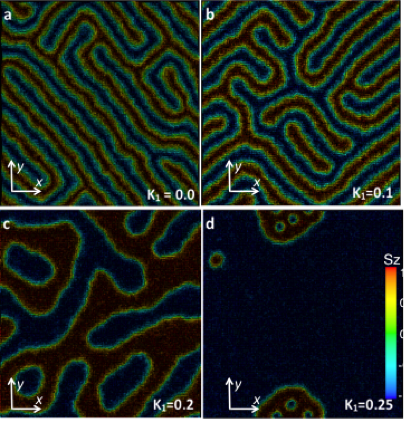
\includegraphics[width=0.5\textwidth,keepaspectratio,natwidth=193,natheight=40]
  {research/yunoki/mc_tx.png}
  \caption{Spin structure of the 2D FM Heisenberg model with the easy axis spin anisotropy (K1) but no external magnetic field.}
  \locallabel{fig:mc_tx}
\end{figure}



%Text for research Results and achievements. Journal-artcile~\cite{sample-journal}.
%Conference-paper~\cite{sample-conference}.
%Invited-talk~\cite{sample-invited}.

%For cross referencing, use \verb|\locallabel| and \verb|\localref| to avoid conflicting names defined by other 
%groups. For example, a figure can be referenced as Figure~\localref{fig:sample-label1}.






\section{Schedule and Future Plan}

\subsection{Large-scale quantum Monte Carlo (QMC) simulations for strongly correlated electrons}

QMC is one of the most powerful methods for quantum simulations in condensed matter physics, especially 
when there is no notorious negative sign problem. We have developed a highly efficient determinant QMC 
code to perform the ground state calculation for the two-dimensional (2D) Hubbard model on the largest lattice 
sites ever using K computer. We plan to continue to develop the determinant based QMC method for strongly 
correlated electrons at zero temperature as well as at finite temperatures, to treat even larger 
lattice sites on exascale computers. One of the challenges for the large-scale simulations is to study 
strongly correlated electrons in three dimensions. We also plan to develop the first principles QMC for 
strongly correlated materials and molecules through international collaboration.

\subsection{Density matrix renormalization group (DMRG) method for quantum dynamics in two dimensions}

The DMRG method was originally proposed and is best performed for the ground state calculations of 
one-dimensional (1D) quantum systems. Owning to high performance computers that are available recently, 
it has become possible to apply the DMRG method not only to the ground state calculations in 2D quantum 
systems but also to the excited state calculations, thermodynamics, as well as real time dynamics. However, 
these dynamical calculations are limited mostly to 1D systems. This is partially because of the exponential 
increase of degrees of freedom to be kept for 2D systems but mainly because of the lack of reliable algorithms 
for thermodynamics and real time dynamics in two dimensions. By combining the kernel polynomial method, 
we plan to develop a new scheme based on the DMRG method for thermodynamics and real time dynamics 
in two dimensions. This will provide the first reliable quantum dynamics calculation for 2D strongly correlated 
quantum systems.

\subsection{First-principles calculations for strongly correlated materials}

Strongly correlated materials are promising as highly functional materials for future technological applications. 
However, the standard first-principles calculations based on the density functional theory (DFT) is not reliable 
because the strong many-body interactions require the treatment that goes beyond the single-particle 
approximation. We plan to develop new first-principles calculation schemes for strongly correlated materials. 
For strongly correlated solid state materials such as transition metal oxides, we apply the many-body cluster 
approximation scheme such as dynamical mean field theory (DMFT), variational cluster approximation (VCA), 
and cluster perturbation theory (CPT), combined with the first-principles calculations based on the DFT. These 
cluster approximation can treat the local electron correlation exactly within a cluster considered and therefore 
is apparently superior to the single-particle approximation. We also plan to apply directly the DMRG method 
as well as the tensor network states to develop an interdisciplinary research on strongly correlated molecules 
such as metalloprotein, in collaboration with Computational Molecular Science Research Team in AICS. 

\subsection{Tensor network scheme for strongly correlated quantum systems}

Although the DMRG method is very powerful for 1D quantum systems, it meets the severe difficulty due to 
the exponential increase of degrees of freedom that have to be kept to guarantee the numerical accuracy 
when it is applied to quantum systems in higher spatial dimensions. This difficulty can be partially overcome 
by aggressively using high performance computers. However, the fundamental resolution has to rely on a 
radical revolution of the algorithm itself. Such a revolution has begun to happen when condensed matter 
physics meets quantum information. Based on the idea of information compression, a tensor network scheme 
has been recently proposed to represent a quantum many-body states with a product of tensors. There still 
exists a big challenge on how to treat the basic tensor operations highly efficiently in large scale calculations. 
We will address this issue to develop the renormalization group method based on tensor network states for 
strongly correlated quantum systems in higher dimensions.

%%% DO NOT EDIT BELOW

\section{Publications}

%\printbibliography[keyword=journal, heading=subbibliography, title={Journal Articles}, prefixnumbers={1-}, resetnumbers=true]
%\printbibliography[keyword=proceedings, heading=subbibliography, title={Conference Papers}, prefixnumbers={2-}, resetnumbers=true]
%\printbibliography[keyword=invited, heading=subbibliography, title={Invited Talks}, prefixnumbers={3-}, resetnumbers=true]
%\printbibliography[keyword=poster, heading=subbibliography, title={Posters and Presentations}, prefixnumbers={4-}, resetnumbers=true]
%\printbibliography[keyword=deliverable, heading=subbibliography, title={Patents and Deliverables}, prefixnumbers={5-}, resetnumbers=true]

\printbibliography[keyword=journal, heading=subbibliography, title={Journal Articles}, resetnumbers=true]
\printbibliography[keyword=proceedings, heading=subbibliography, title={Conference Papers}]
\printbibliography[keyword=invited, heading=subbibliography, title={Invited Talks}]
\printbibliography[keyword=poster, heading=subbibliography, title={Posters and Presentations}]
\printbibliography[keyword=deliverable, heading=subbibliography, title={Patents and Deliverables}]

\end{refsection}
